
%In here will be the testings and thought process of the convergence results

%In here discuss the extensive testing on how fast computations take and how fine the grid for the finite difference method needs to be so that a sufficient convergence can be observed.

%If I ever get around to it, refere to the results of convergence testing though Python is.

%(Show the results of a convergence analysis.)
%    Maybe use the epsilon delta thing from sci. comp class.
%    Then this section will be mostly an explain of what the epsilon delta 
%        thing and then a few graphs of the different convergence results
%    run the different tests for different t values???

\section{Convergence Results}


The accuracy of this method depends on the grid size used. A convergence analysis is done to observe at what resolution sufficient accuracy is seen. This is done by comparing the relative error in average $M$ between two solutions with different $\Delta x$. We call this difference $\delta$, which we compute as
\begin{equation} \label{equ:converg_delta}
    \delta_k = \frac{\left|\overline{M}_{k+1} - \overline{M}_{k} \right|}{\overline{M}_{k+1}}
\end{equation}
where $\overline{M}_{k}(t)$ is the average biomass at time $t$, solved with $\Delta x = 2^{-k}$. Figure \ref{fig:converg_average} was computed using (\ref{equ:converg_delta}) with $k = 7,8,...,14$. 


\begin{figure}[!htb]
    \begin{center}
        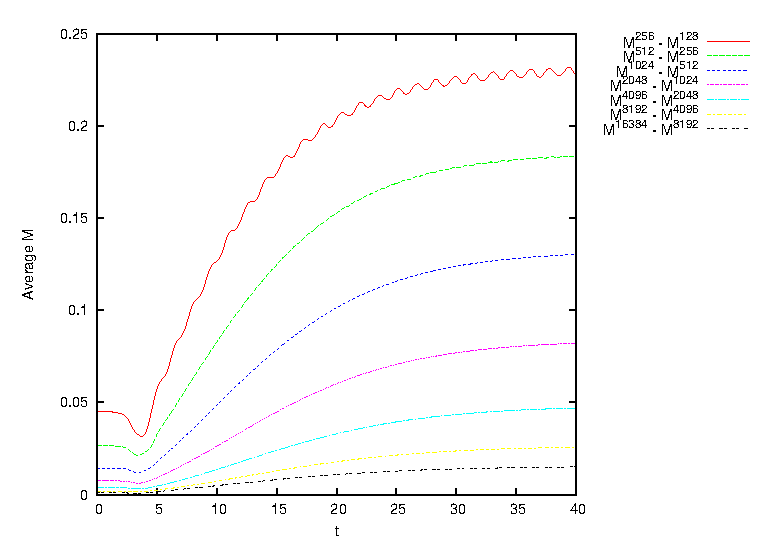
\includegraphics[scale=0.7]{converg_total.eps}
        \caption{Comparison of mean $M$, using (\ref{equ:converg_delta}) with $i = 7,8,...,14$}
        \label{fig:converg_average}
    \end{center}
\end{figure}

This convergence analysis shows a relative error less then $0.02\%$ can be achieved by using $\Delta x = 2^{-13}$. This is considered an sufficient accuracy.
%!%
%!%
%!% FIND A SOURCE THAT SAYS THIS IS ACCURATE ENOUGH
%!%
%!%

A second convergence result can be done by instead comparing each gridpoint between solutions. If we define 
\begin{equation} \label{equ:converg_sigma}
    \sigma_k(t) = 2^{-k} \sum_{i,j} |M^{k+1}(t, x_i, y_j) - M^k(t, x_i, y_i)|,
\end{equation}
and 
\begin{equation} \label{equ:converg_rho}
    \rho_k = \frac{1}{n(T)} \sum_{\forall t \in T} \sigma_k(t).
\end{equation}
In (\ref{equ:converg_sigma}), $M^{k}(t,x_i,y_i)$ refers to the biomass when solved with $\Delta x = 2^{-k}$ at time t and gridpoint $(x_i, y_i)$. The value of $\sigma_k(t)$ is the average difference between related gridpoints of solutions solved with different $\Delta x$ values at a specific time $t$. In (\ref{equ:converg_rho}), $n(T)$ refers to the cardinality of $T$, which is the number of outputted times we have. The value of $\rho$ is the average difference across all $t \in T$. 
%!% Reference the nonexistance figure here.

\begin{figure}[!htb]
    \begin{center}
  %!% Make this figure exist      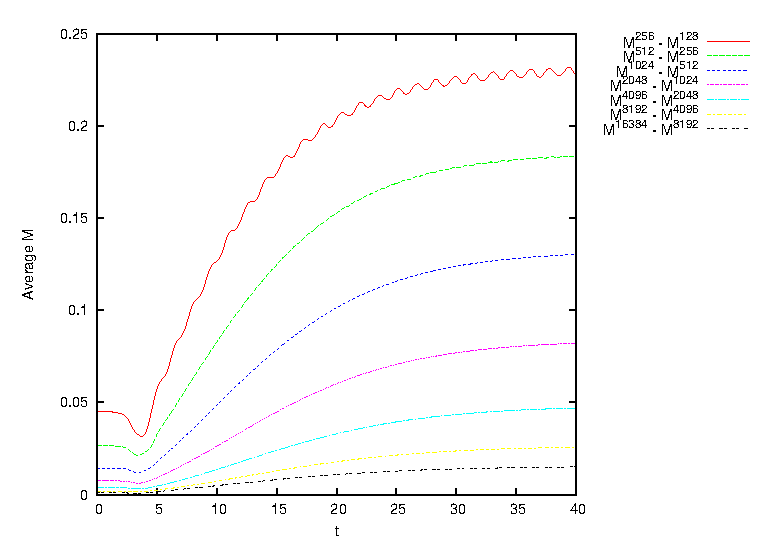
\includegraphics[scale=0.7]{converg_total.eps}
        \caption{Graph of $\rho_k$, for $k = 7,8,...,13$ and $T = 0,2,...,40$}
        \label{fig:converg_rho}
    \end{center}
\end{figure}

This can be extended to check convergence in $\Delta t$ by defining
\begin{equation} \label{equ:converg_rhoBar}
    \overline{\rho}_{\tau} = \sum_k \rho^{\tau}_k
\end{equation}
where $\rho^{\tau}_k$ is the same computations for (\ref{equ:converg_rho}) done with $\Delta t = \tau$.

%!% Add a table of values for \rho^{\tau}






